\documentclass{article}
\usepackage{amsmath}
\usepackage{amssymb}
\usepackage{array}
\usepackage{amsmath}
\usepackage{tikz}
\usetikzlibrary{automata, positioning}

\begin{document}

\begin{flushleft}

\end{flushleft}

\section*{Problem 1}

\[
s_n = \sum_{i=2}^{n} \frac{1}{i^2 - 1} = \frac{(n-1)(3n+2)}{4n(n+1)}
\]

\subsection*{Proof by Induction}

We will prove the statement 
\[
s_n = \sum_{i=2}^{n} \frac{1}{i^2 - 1} = \frac{(n-1)(3n+2)}{4n(n+1)}
\]
using mathematical induction.

\subsubsection*{Base Case}
For \( n = 2 \):

\[
s_2 = \sum_{i=2}^{2} \frac{1}{i^2 - 1} = \frac{1}{3}
\]

\[
\frac{(2-1)(3 \cdot 2 + 2)}{4 \cdot 2 \cdot (2+1)} = \frac{1 \cdot 8}{4 \cdot 2 \cdot 3} = \frac{8}{24} = \frac{1}{3}
\]

So, the base case holds true.

\subsubsection*{Inductive Step}
Assume that the statement is true for some \( i = 2, 3, 4, ..., n \)

\[
s_i =  \frac{(i-1)(3i+2)}{4i(i+1)}
\]

\subsubsection*{Show that}

\[
s_{n+1} =  \frac{n(3n+5)}{4(n+1)(n+2)}
\]

Using the inductive hypothesis:

\[
s_{n+1} =  \sum_{i=2}^{n+1} \frac{1}{i^2 - 1} = s_n + \frac{1}{(n+1)^2 - 1}
\]

\[
s_{n+1} = \frac{(n-1)(3n+2)}{4n(n+1)} + \frac{1}{(n+1-1)(n+1+1)} = \frac{(n-1)(3n+2)}{4n(n+1)} + \frac{1}{n(n+2)}
\]

To add these fractions, find a common denominator:

\[
s_{n+1} = \frac{(n-1)(3n+2)(n+2) + 4(n+1)}{4n(n+1)(n+2)}
\]

Simplifying the numerator:

\[
s_{n+1} = \frac{(3n^2-n-2)(n+2)+4(n+1)}{4n(n+1)(n+2)}
\]

\[
s_{n+1} = \frac{(3n^3+6n^2-n^2-2n-2n-4)+4n+4}{4n(n+1)(n+2)}
\]

\[
s_{n+1} = \frac{(3n^3+5n^2-4n-4)+4n+4}{4n(n+1)(n+2)}
\]

\[
s_{n+1} = \frac{3n^3+5n^2}{4n(n+1)(n+2)}
\]

\[
s_{n+1} = \frac{n^2(3n+5)}{4n(n+1)(n+2)}
\]

\[
s_{n+1} = \frac{n(3n+5)}{4(n+1)(n+2)}
\]




This matches the form of \( \frac{n(3n+5)}{4(n+1)(n+2)} \), confirming the statement holds for \( n+1 \).

By the principle of mathematical induction, the statement is true for all \( n \geq 2 \).

\section*{Problem 2}

Given sets \( A \) and \( B \):

\[
A = \{2, 3, 5, 7\}
\]

\[
B = \{2, 4, 5, 8, 9\}
\]

The universal set \( U \) is:

\[
U = \{0, 1, 2, 3, 4, 5, 6, 7, 8, 9, 10\}
\]

First, we find the complement of \( B \), denoted as \( \overline{B} \):

\[
\overline{B} = U - B = \{0, 1, 3, 6, 7, 10\}
\]

Next, we find the union of \( A \) and \( \overline{B} \):

\[
A \cup \overline{B} = \{2, 3, 5, 7\} \cup \{0, 1, 3, 6, 7, 10\} = \{0, 1, 2, 3, 5, 6, 7, 10\}
\]

Then, we find the complement of \( A \cup \overline{B} \), denoted as \( \overline{A \cup \overline{B}} \):

\[
\overline{A \cup \overline{B}} = U - (A \cup \overline{B}) = \{4, 8, 9\}
\]

Thus, the set \( S \) is:

\[
S = \{4, 8, 9\}
\]

\section*{Problem 3}

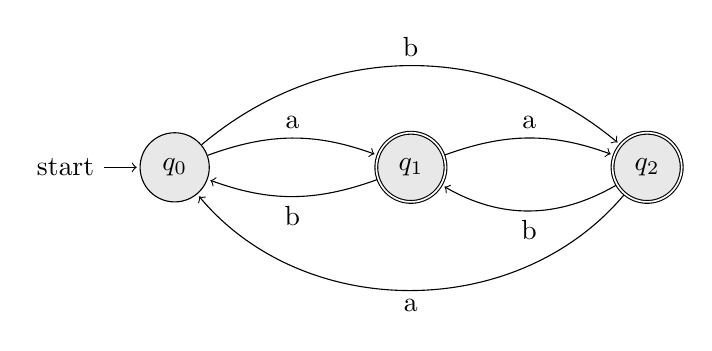
\begin{tikzpicture}[shorten >=1pt,node distance=3cm,auto]
  \tikzstyle{every state}=[fill={rgb:black,1;white,10}, text=black]

    \node[state,initial]   (q_0)                    {$q_0$};
    \node[state, accepting]           (q_1)  [right of=q_0]    {$q_1$};
    \node[state,accepting] (q_2)  [right of=q_1]    {$q_2$};

    \path[->]
     (q_0)
          edge [bend left=40]  node {b}    (q_2)
          edge [bend left=20]  node {a}    (q_1)
    (q_1) 
          edge [bend left=20]  node {b}  (q_0)
          edge [bend left=20]  node {a}    (q_2)
    (q_2) edge [bend left=30]  node {b}    (q_1)
          edge [bend right= -50]  node {a}    (q_0);
\end{tikzpicture}

\section*{Problem 4}
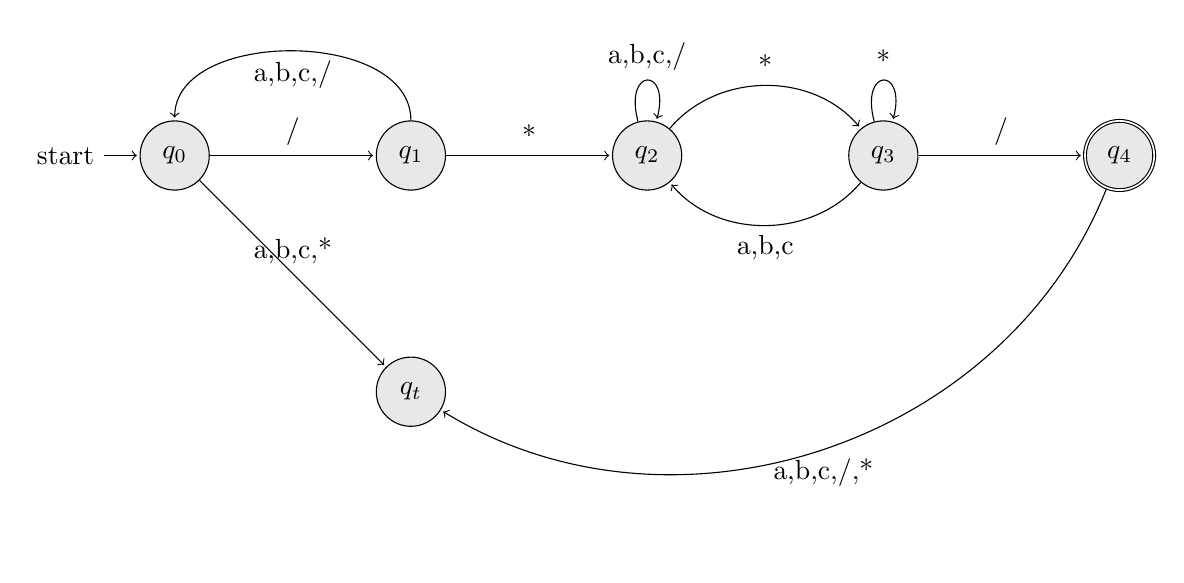
\begin{tikzpicture}[shorten >=1pt,node distance=3cm,on grid,auto]
  \tikzstyle{every state}=[fill={rgb:black,1;white,10}, text=black]

    \node[state,initial]   (q0)                    {$q_0$};
    \node[state]           (q1)  [right of=q0]    {$q_1$};
    \node[state]           (q2)  [right of=q1]    {$q_2$};
    \node[state]           (q3)  [right of=q2]    {$q_3$};
    \node[state,accepting] (q4)  [right of=q3]    {$q_4$};
    \node[state]           (qt)  [below of=q1]    {$q_t$};

    \path[->]
    (q0) edge [above] node {/} (q1)
         edge [above] node {a,b,c,*} (qt)
    (q1) edge [above] node {*} (q2)
         edge [bend right=90] node {a,b,c,/} (q0)
    (q2) edge [loop above] node {a,b,c,/} ()
         edge [bend left=50, above] node {*} (q3)
    (q3) edge [loop above] node {*} ()
         edge [above] node {/} (q4)
         edge [bend left=50, below] node {a,b,c} (q2)
    (q4) edge [bend left=50, below] node {a,b,c,/,*} (qt);

    
\end{tikzpicture}


\section*{Problem 5}



\[
\begin{array}{rcl}
S & \rightarrow & 0A \ | \ 1B \ | \ \lambda \\
A & \rightarrow & 1A \ | \ 0B \ | \ \lambda \\ 
B & \rightarrow & 0B \ | \ 1A
\end{array}
\]


\section*{Problem 6}

The language \( L \) generated by the grammar \( G \) is:

\[
L = \{ w \colon |w| \mod 4 \neq 0 \}
\]

### Short Description of the Conclusion

The outputs of the grammar can be a sequence of `a` or `a`s, but it follows one of these three rules: the length of `a`s is \( 4q + 1 \), \( 4q + 2 \), or \( 4q + 3 \). This means the length of `a`s is not divisible by 4, and the remainder of this division could be 1, 2, or 3, but not 0. Therefore, the length of the `a`s mod 4 is not equal to zero.

#### Examples of Derivations

1. Derivations for \( S \rightarrow A \):
   \[
   \begin{aligned}
   & S \rightarrow A \rightarrow a \\
   & S \rightarrow aaaaA \rightarrow aaaaa \\
   & S \rightarrow aaaaA \rightarrow aaaaaaaaA \rightarrow aaaaaaaaa \\
   & S \rightarrow aaaaA \rightarrow aaaaaaaaA \rightarrow aaaaaaaaaaaaA \rightarrow aaaaaaaaaaaaa \\
   & \text{and so on.}
   \end{aligned}
   \]

2. Derivations for \( S \rightarrow B \):
   \[
   \begin{aligned}
   & S \rightarrow B \rightarrow aa \\
   & S \rightarrow aaaaB \rightarrow aaaaaa \\
   & S \rightarrow aaaaB \rightarrow aaaaaaaaB \rightarrow aaaaaaaaaa \\
   & S \rightarrow aaaaB \rightarrow aaaaaaaaB \rightarrow aaaaaaaaaaaaB \rightarrow aaaaaaaaaaaaaa \\
   & \text{and so on.}
   \end{aligned}
   \]

3. Derivations for \( S \rightarrow C \):
   \[
   \begin{aligned}
   & S \rightarrow C \rightarrow aaa \\
   & S \rightarrow aaaaC \rightarrow aaaaaaa \\
   & S \rightarrow aaaaC \rightarrow aaaaaaaaC \rightarrow aaaaaaaaaaa \\
   & S \rightarrow aaaaC \rightarrow aaaaaaaaC \rightarrow aaaaaaaaaaaaC \rightarrow aaaaaaaaaaaaaaa \\
   & \text{and so on.}
   \end{aligned}
   \]


\end{document}
